\documentclass[12pt,dvipdfmx,svgnames,uplatex,aspectratio=169]{beamer}
% \documentclass[12pt,dvipdfmx,svgnames,uplatex,aspectratio=169,handout]{beamer}
%
% ===========================================
% 図・表関係
% ===========================================
% \usepackage[draft]{graphicx}
\usepackage{graphicx}
\graphicspath{{./pics/}}  % \includegraphicsで参照するディレクトリ
%
% ===========================================
% 参考文献
% ===========================================
\usepackage[url=false,isbn=false,doi=false]{biblatex}
% \addbibresource{./bib_textbooks.bib}  % 教科書など
% \addbibresource{./bib_articles.bib}  % 論文など
%
% ===========================================
% 独自スタイルの導入
% ===========================================
\usepackage{/home/ryo/.config/LaTeX/mystyle_beamer}
\newcommand{\git}[1]{{\colorbox{WhiteSmoke}{\texttt{\textbf{#1}}}}}  % gitコマンドを薄い灰色の背景とtypewriterフォントで表記
%
% ===========================================
% 表紙の記述
% ===========================================
\title{非情報系理系院生のための \\
  モダンな開発環境づくり}
\subtitle{その1. Git/GitHubを使ったソースコード管理}
\author{荒木 亮}
\institute{阪大院基礎工・後藤研}
\date{\today}

% +++++++++++++++++++++++++++++++++++++++++++
% 本文
% +++++++++++++++++++++++++++++++++++++++++++

\begin{document}
\frame{\maketitle}
\begin{frame}{もくじ}
  \tableofcontents
\end{frame}

% ===========================================
% 以下,スライドを記述する
% ===========================================
\section{目標}
\begin{frame}{\insertsection}
  \begin{screen}
    \centering
    ソースコードやLaTeX文書のバージョンを,Git/GitHubで管理する
  \end{screen}

  \begin{itemize}
    \item Gitに初めて触れる人が,「ファイル名に日付をつけてバックアップ」\\をGitで代替できるようになることをめざす
  \end{itemize}

  \begin{alertblock}{説明しないこと}
    \begin{itemize}
      \item \git{branch} を使った同時並行的な開発
      \item \git{pull request} を使ったチームでの開発
      \item その他色々ややこしいコマンド
    \end{itemize}
  \end{alertblock}
\end{frame}

\section{Gitの構造}
\begin{frame}{\insertsection}
  \centering
  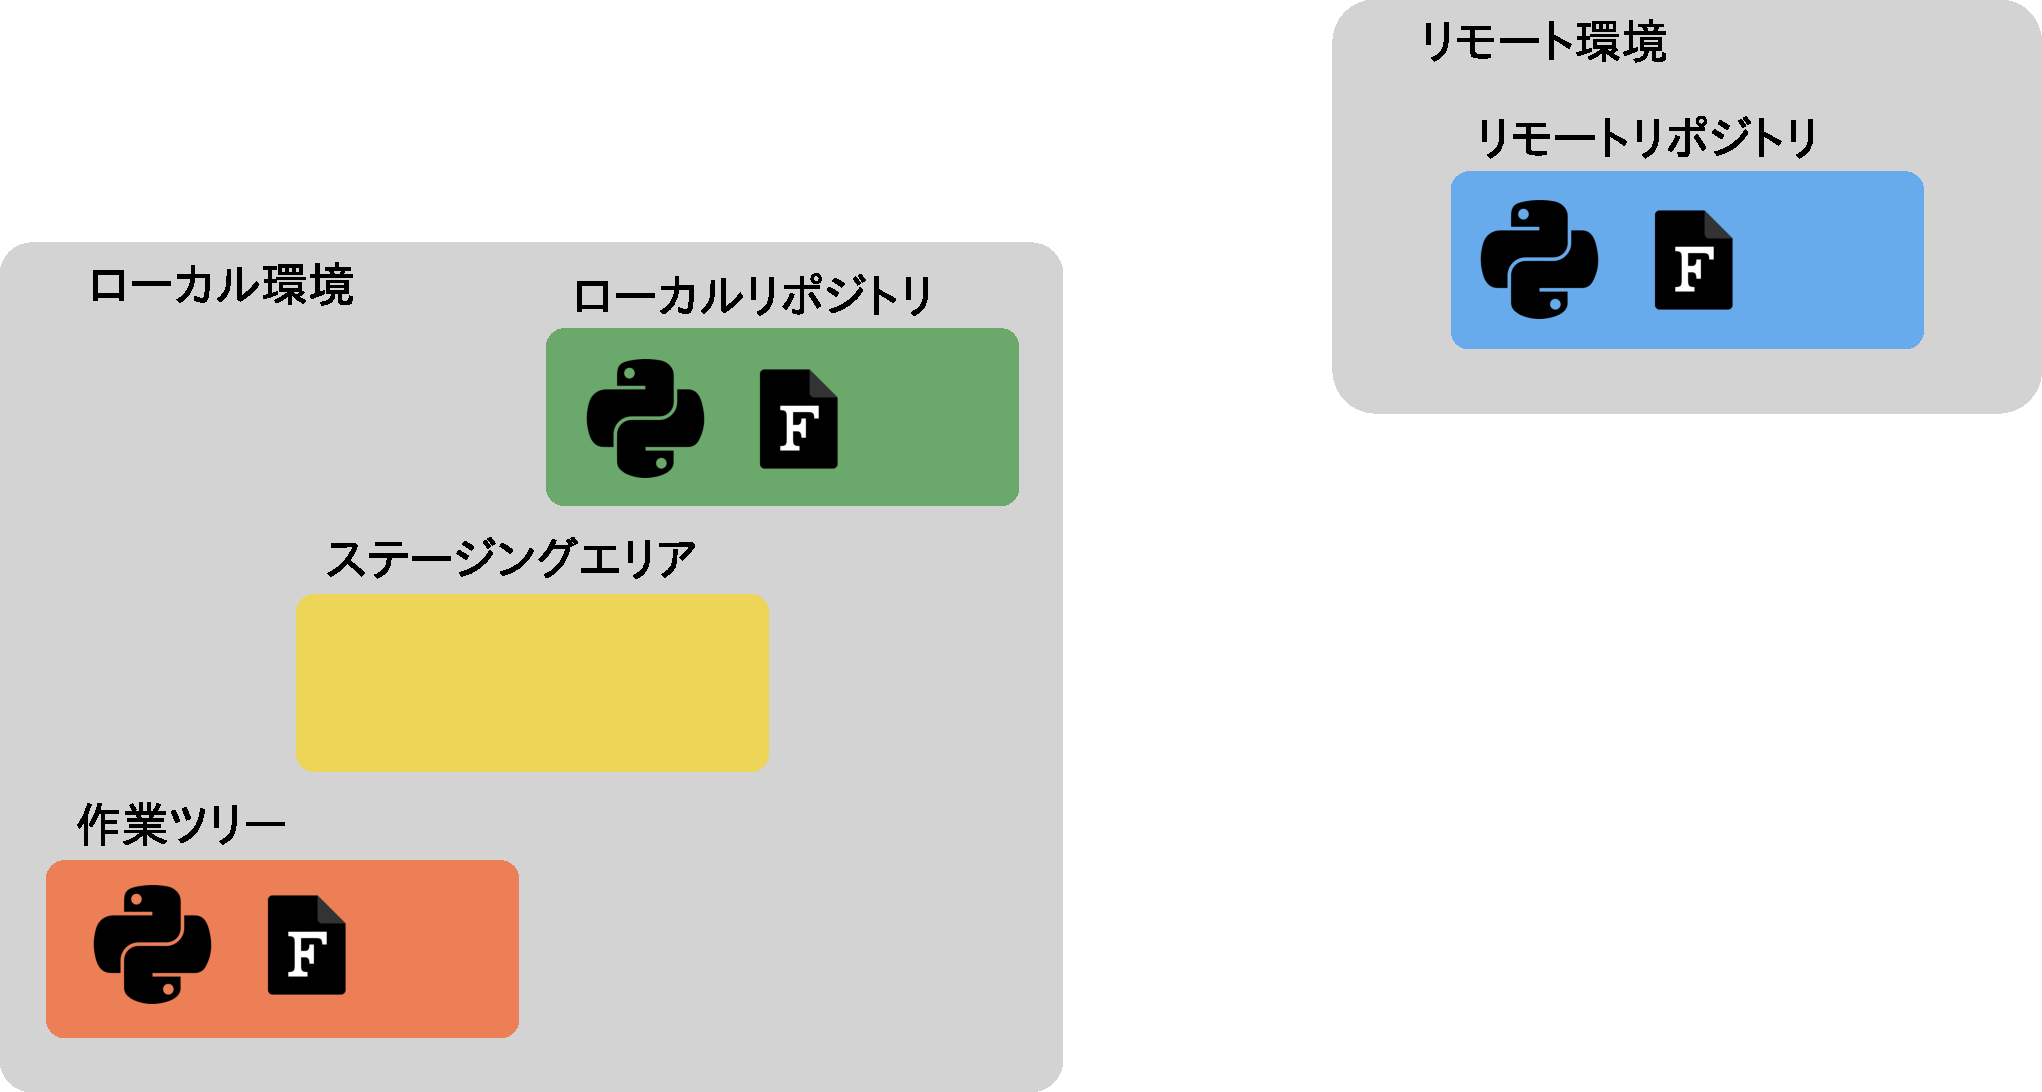
\includegraphics[bb=0.000000 0.000000 979.966736 524.329163, width=120mm]{./pics/git_structure.pdf}
  \begin{flushright}
    \scriptsize{Figures from: \href{https://icon-icons.com/ja/}{icon-icons.com}}
  \end{flushright}
\end{frame}

\begin{frame}{\insertsection}
  \begin{block}{作業ツリー}
    作業をおこなうディレクトリ.普通の意味の「フォルダ」
  \end{block}
  \begin{block}{ステージングエリア}
    作業ツリーで編集したファイルの変更点を「とりあえず」保管しておく場所
  \end{block}
  \begin{block}{ローカルリポジトリ}
    ステージングエリアにある変更点を「コミット」としてまとめ,記録する場所
  \end{block}
  \begin{block}{リモートリポジトリ}
    ソースコードなどをまとめた「リポジトリ」を保存・公開する場所
  \end{block}
\end{frame}

\section{Gitのコマンド}
\begin{frame}{\insertsection}
  \centering
  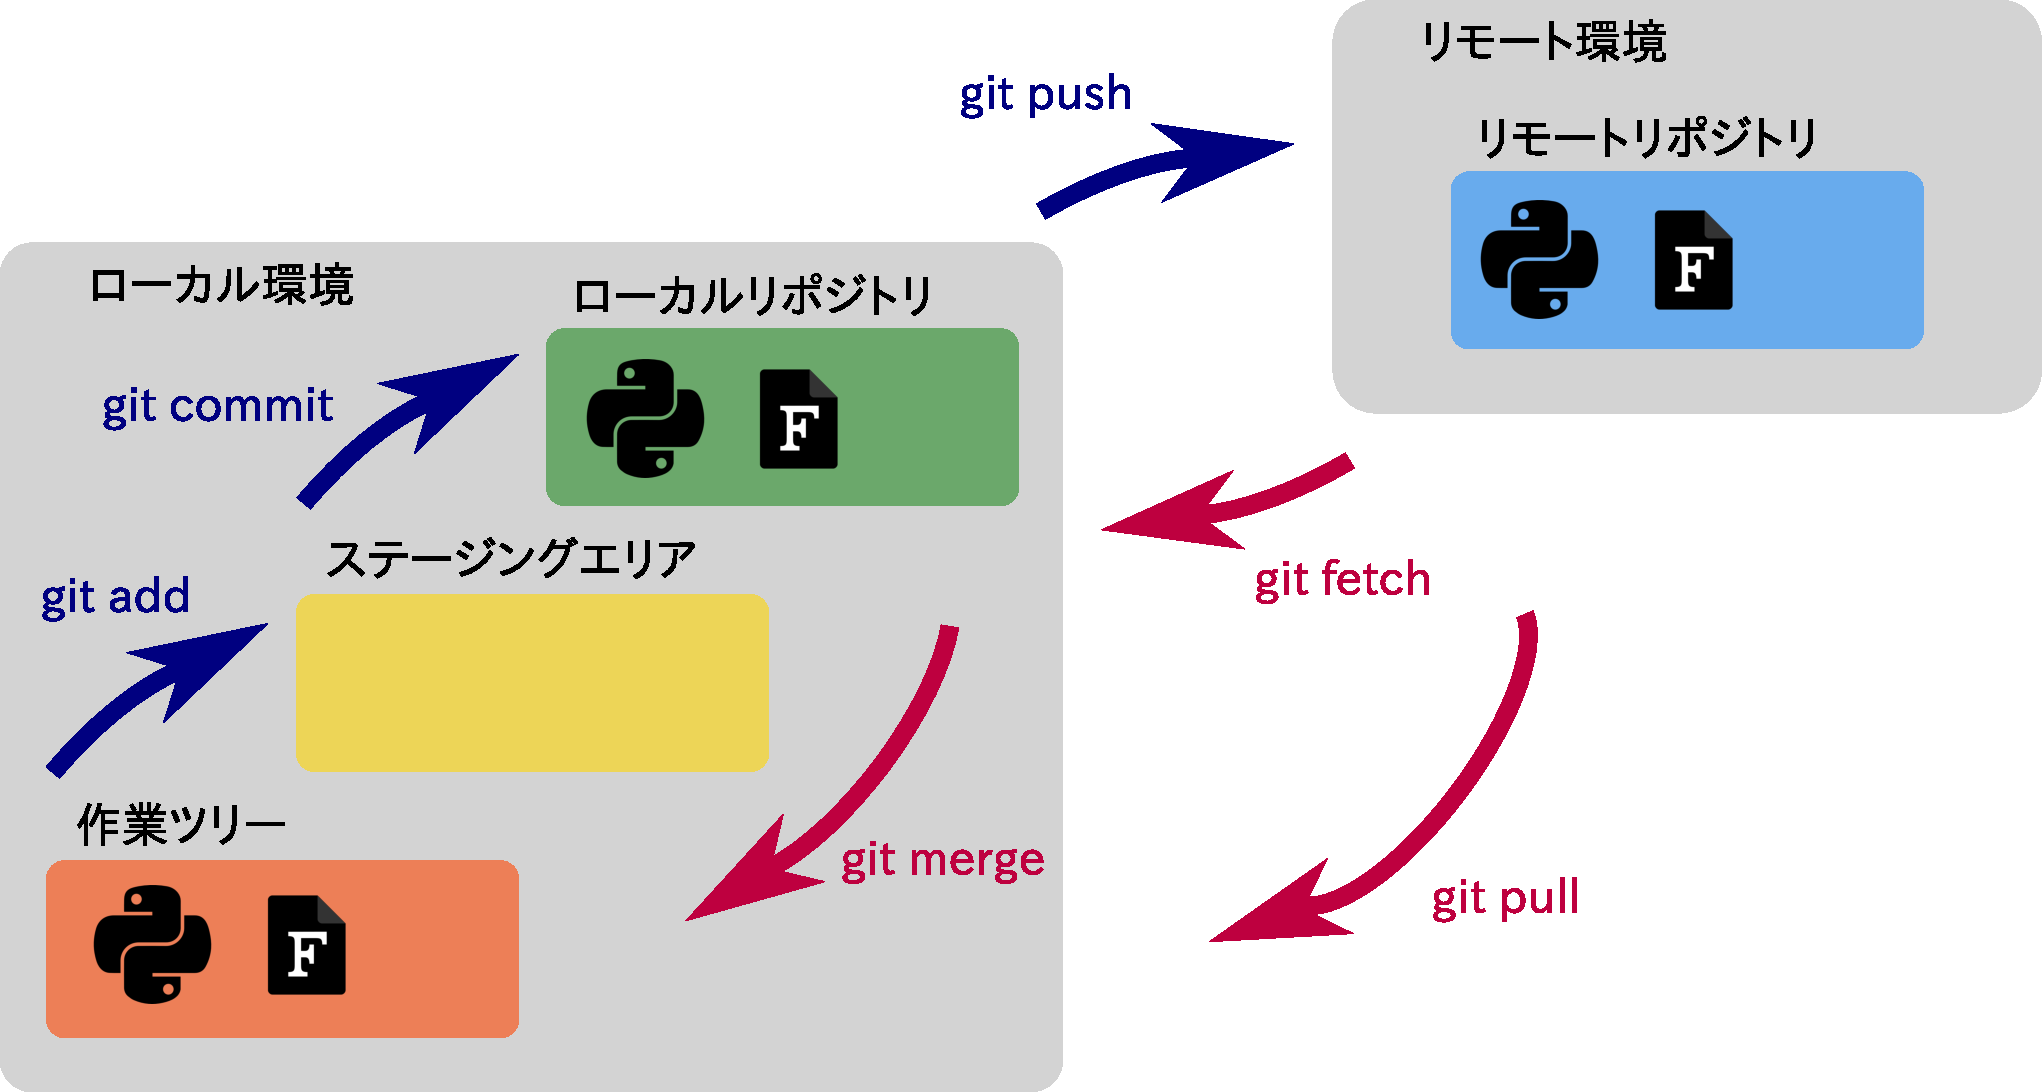
\includegraphics[bb=0.000000 0.000000 979.966736 524.329163, width=120mm]{./pics/git_structure_command.pdf}
  \begin{flushright}
    \scriptsize{Figures from: \href{https://icon-icons.com/ja/}{icon-icons.com}}
  \end{flushright}
\end{frame}

\begin{frame}{\insertsection}
  \begin{block}{\git{git add}}
    作業ツリーで編集したファイルの変更点をステージングエリアに追加
  \end{block}
  \begin{block}{\git{git commit}}
    ステージングエリアにある変更点の集合をローカルリポジトリに記録
  \end{block}
  \begin{block}{\git{git push}}
    ローカルリポジトリに記録されたコミット群をリモートリポジトリに送信
  \end{block}
  \begin{block}{\git{git pull}}
    リモートリポジトリの最新の情報をローカルリポジトリに適用
  \end{block}
\end{frame}

\section{分散型バージョン管理}
\begin{frame}{\insertsection}
  \begin{columns}[c] % 中央をあわせる
    \begin{column}{0.5\textwidth}
      \includegraphics[bb=0.000000 0.000000 600.000000 316.000000, width=60mm]{./pics/multi.png}

      \includegraphics[bb=0.000000 0.000000 589.565143 347.771411, width=60mm]{./pics/intro2_2.png}

      \scriptsize{Figures from: \href{https://owncloud.jp}{ownCloud},\href{https://backlog.com/ja/git-tutorial/}{サルでも分かるGit入門}}
    \end{column}
    \begin{column}{0.5\textwidth}
      \begin{block}{自動更新(クラウドサービス)}
        変更箇所を自動でリモートに送る
      \end{block}
      \begin{block}{commit(Git/GitHub)}
        変更箇所を任意の粒度でまとめ,名前やコメントをつけて管理するもの
        \begin{itemize}
          \item 編集履歴がわかりやすい
          \item 昔の状態の確認や巻き戻しが簡単
          \item 編集が競合したとき,解決が簡単
        \end{itemize}
      \end{block}
    \end{column}
  \end{columns}
\end{frame}

\section{なぜGitを使うのか}
\begin{frame}{\insertsection}
  \begin{itemize}
    \item 自動で保存されてしまうクラウドサービスだと…
    \item[] 「前の状態に戻したいんだけど,あれっていつのバージョンだっけ?」
    \item 古い状態を記録しておけないと…
    \item[] 「今はこの関数やサブルーチンを使ってないけど,また使うかも\\しれないしとりあえずコメントアウトして残しておこう」
    \item 共同作業で競合がおきてしまうと…
    \item[] 「今からこのファイル編集するから触らないでね!」
    \item[] 「最新のファイルってどこに置いてる?」
  \end{itemize}

  \begin{block}{Gitを使うべきでないファイル}
    \begin{itemize}
      \item 一度作成したらもう編集しないデータ(実験結果,計算データ)
      \item[] \(\to\)(普通の意味での)バックアップで対処する
      % \item ソースコード,論文データなど,継続的に改良していくデータ → (Gitなどを使った)バージョン管理
    \end{itemize}
  \end{block}
\end{frame}

\section{今日から始めるGit生活}
\begin{frame}{\insertsection}
  \begin{enumerate}
    \item GitHubでアカウント作成
    \item Education planの作成
    \begin{itemize}
      \item[※] 「非公開リポジトリ」が無制限に作成できる
    \end{itemize}
    \item 研究用リポジトリの作成
    \begin{itemize}
      \item[※] 別のプロジェクトには別のリポジトリを利用:全て一つの場所で管理しない
    \end{itemize}
    \item コードを保存しているディレクトリを登録
    \item ファイル編集\(\to\) \git{add} \(\to\) \git{commit} \(\to\) \git{push}
    \begin{itemize}
      \item[※] 見返してわかりやすい「commitメッセージ」をつける
    \end{itemize}
    \item GitHubのページを確認し,コードが変更されていることを確認
  \end{enumerate}
\end{frame}

\section{便利なGitコマンド}
\begin{frame}{\insertsection}
  \begin{block}{\git{git checkout .}}
    作業ツリーの変更点を破棄,ステージングエリアの状態を回復
  \end{block}
  \begin{block}{\git{git stash}}
    現在の作業内容を退避し,ステージングエリアの状態を回復

    対比した状態は任意に回復できる
  \end{block}
  \begin{block}{\git{git commit --amend}}
    一旦ローカルリポジトリに登録したコミットを修正
  \end{block}
  \begin{block}{\git{git reflog}}
    \git{git ***}のコマンドログを確認
  \end{block}

  % その他, \git{git revert} \git{git reset}
  % gitコマンドへのオプション,\texttt{.gitignore}
\end{frame}

\section{リンク集}
\begin{frame}{\insertsection}
  \begin{block}{よみやすい順}
    \begin{itemize}
      \item \href{https://backlog.com/ja/git-tutorial/}{サルでもわかるGit入門}
      \begin{itemize}
        \item 「まずGitの勉強をしたい」ときにおすすめします.豊富な(かわいい)絵で説明されているので,かなりとっつきやすいと思います.
      \end{itemize}
      \item \href{https://www.slideshare.net/matsukaz/git-28304397}{いつやるの?Git入門 v1.1.0}
      \item \href{https://git-scm.com/book/ja/v2}{Pro Git book(日本語版)}
      \begin{itemize}
        \item 有名なGitの書籍で,オンラインで読むことができます(PDFもダウンロードできます).Linuxでのコマンド操作をベースに解説されており,やや敷居が高いかもしれませんが,とてもよい資料と思います.
      \end{itemize}
      \item \href{https://www.slideshare.net/kotas/git-15276118}{こわくない Git}
    \end{itemize}
  \end{block}
  何か疑問・質問があればslackの \texttt{\#50\_github} まで!
\end{frame}

\end{document}
